\section{Strategien und Kommunikation}

\subsection{Client}

Der Client erwartet beim Aufrufen eine zusätzliche Eingabe des Benutzers. Dabei handelt es sich um ''Client'' und zwei Zahlen. Die erste Zahl gibt an wie oft 
eine Strategie ausgeführt werden soll, es werden nur Integer akzeptiert. Mit der zweiten Zahl wird die Strategie ausgewählt, es werden nur Integer im Bereich von 
0 -6 akzeptiert. \\Nach der Eingabe wird die passende Strategie aufgerufen und in einer for-Schleife entsprechend oft der Eingabe ausgeführt.

\subsection{Server}

Der Server ist eine Kindklasse, die public von TCPserver geerbt hat. Der Server wurde um die Variablen world und Shootresult erweitert, welche private sind. 
Eine Funktion des Servers ist myResponse, Sie bekommt als Eingabe einen String der vom Client geschickt wird, 
vergleicht die Koordinaten mit dem internen Spielfeld und gibt einen String als Antwort zurück. Es gibt folgende Antwortmöglichkeiten: ''Water'', ''ShipHit'', 
ShipDestroyed'', ''AllShipsDestroyed'', ''GameOver'', abhqngig vom internen SPielfeld. Schickt der Client als String ''Restart'' erstellt der Server ein neues Spielfeld und das Spiel beginnt von neuem.

\subsection{Protokoll Server}
Zur Kommunikation zwischen Server und Client läuft nach folgendem Protokoll ab.\\
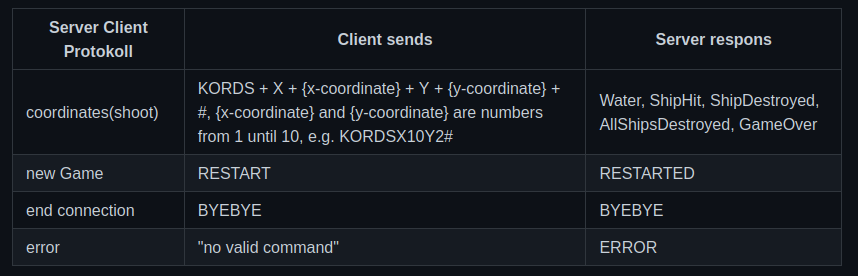
\includegraphics[scale=0.5]{ProtokollServer.png}\\

Wenn der Client eine Strategie ausgeführt, wird bei jedem Schuss ein String mit den zu beschießenden an den Server gesendet und der Server überprüft den Status auf dem internen Spielfeld und sendet eine Antwort in Form eines Strings zurück (siehe Tabelle Zeile 1 Spalte 2).
Um ein neues Spiel zu beginnen, muss der Client den String \\''RESTART'' an den Server senden, dieser startet dann ein neues Spiel und sendet den String ''RESTARTED'' an den Client zurück. Um die Verbindung zu beenden, \\sendet der Client ''BYEBYE'', der Server sendet ''BYEBYE'' zurück und beendet die Verbindung.
Sendet der Client einen String, der nicht dem Protokoll entspricht, antwortet der Server mit ''ERROR''. 

\subsection{Strategien}
Zum beschießen des erzeugten Spielfelds werden 7 unterschiedliche Strategien verwendet.

\subsubsection{Bruteforce}

Die Strategie BruteForce schießt nacheinander auf alle Zeilen und alle Spalten, bis der Server mitteilt, dass alle Schiffe zerstört sind. Bei jedem Schuss wird ein Schuss Zähler hochgezählt, dieser wird am Ende der Strategie zurückgegeben.

\subsubsection{BruteforceDiagonal}

Die Strategie schießt nacheinander auf alle Felder im Spiel. Die Reihenfolge der Schüsse ist diagonal angeordnet. Die Strategie wird beendet, wenn der Server mitteilt, dass alle Schiffe zerstört sind. Bei jedem Schuss wird ein Schuss Zähler hochgezählt, dieser wird am Ende der Strategie zurückgegeben.

\subsubsection{Randshoot}

Bei dieser Strategie wird mittels der rand()-Funktion die Koordinaten von 1 bis 10 für
beide per Zufall ausgewählt und eine Anfrage mit diesen beliebigen Koordinaten an den
Server geschickt. Doppelungen von Anfragen oder mehr als zweimal können auftreten,
da nicht gespeichert wird, ob das Feld bereits angefragt wurde oder nicht.

\subsubsection{RandshootiS}

Diese Strategie ist die Erweiterung zu der randshoot-Strategie. Die Generierung der
Koordinaten erfolgt wie bei der ersten Strategie. Ergänzend hinzugekommen ist, dass
diese Strategie die Anfragen in einem zweidimensionalen Feld abspeichert und nach
einer erneuten Generierung prüft, ob diese Koordinaten bereits angefragt wurden. Ist
dies der Fall, werden neue Koordinaten generiert. Es erfolgt dann keine neue Anfrage an
den Server bei bereits angefragten Koordinaten, die bereits vorher schon angefragt
wurden. Fällt das Ergebnis dieser Anfragen negativ aus, so wird eine Anfrage an den
Server gestellt. Wird eine Anfrage gestellt, wird der Wert der Koordinaten in der Matrix
(2D-Feld) gemäß der boolschen Wahrheitswerte von „false“ auf „true“ geändert.

\subsubsection{Intellistrat}

Die intelligente Strategie schießt nacheinander (Zeile und Spalte) auf das Spielfeld. Nach jedem Schuss auf ein Feld wird in einer Wahrheitswertmatrix die 
beschossene Position markiert. Wenn die Strategie einen Treffer erzielt, zerstört Sie zuerst das getroffene Schiff. Dies tut Sie, indem Sie auf die horizontalen 
und vertikalen Nachbar Felder schießt, bis ihr der Server mitteilt, dass das Schiff zerstört ist. Im Anschluss maskiert Sie die beschossenen und die umliegenden 
Felder in der Wahrheitswertmatrix, da dort kein weiteres Schiff liegen kann. Bei jedem Schuss wird ein Schuss Zähler hochgezählt, dieser wird am Ende der 
Strategie zurückgegeben.

\subsubsection{IntellistratDiagonal}

Die diagonale intelligente Strategie ist auf der einfachen intelligenten Strategie aufgebaut. Der einzige unterscheid besteht darin, dass Sie nur jede zweite 
diagonale Reihe beschießt. Dies ist möglich, da keine Schiffe existieren, die nur ein Feld groß sind.


\subsection{Verbrannte Felder}

\subsection{Spielfeldverwaltung}

Die SpielFeldverwaltung setzt sich aus folgenden Funktionen und einer Klasse zusammen,
void restart, enum Feldstatus, string shootPos, Feldstatus shootline, Feldstatus Nachbar und der Klasse SpielfeldVerwaltung.
Die Funktion restart wird vom Client benötigt um dem Server mitzuteilen dass das Spiel neugestartet werden soll und shootpos wird verwendet um dem Server mitzuteilen auf welches Feld 
geschossen werden soll und gibt den Antwortstring des Servers zurück. Unter Feldstatus sind die Enums gespeichert die von der Klasse Spielfeldverwaltung benutzt werden, Erklärung 
folgt. Die Funktionen Nachbar und Shootline suchen und zerstören ein Schiff komplett wenn ein Treffer gelandet wurde. Sie Funktionieren nach dem Prizip der Funktion Neigbour welche 
in der Datei Intellistrat.C verwendet wird und machen sich die Methoden der Klasse zur nutze. Wird ein Schiff getroffen so wird die Funktion Nachbar aufgerufen, sie benötigt als 
Übergabeparameter die x- und die y- Koordinate, die Anzahl der gezählten Schritte, den TCPclient und eine Referenz auf die aktuelle Instanz der Klasse. Dann wird viermal die Funktion 
Shootline aufgerufen, Shootline benötigt die eben genennte Übergabeparameter und zusätzlich noch zwei Additionsvariablen. In der Funktion werden dann die Additionsvariablen in einer 
do-while Schleife auf die x- und y- Variablen aufaddiert, solange der Server ShipHit als Rückgabe liefert. Dies führt dazu das in eine Richtung geschossen wird. Wenn Wasser als 
Rückgabewert kommt wird die Funktion beendet und Nachbar ruft Shootline solange auf bis alle vier Richtungen ausprobiert wurden bzw. bis das Schiff zerstört wurde, tritt dies schon 
nach dem ersten aufgerufen von Shootline auf wird die Funktion Nachbar ebenfalls beendet.

Die gleichnahmige Klasse SpielfeldVerwaltung besitz ein \newline eindimensionales Array Spielfeld mit 100 Variablen des Typs Enum
(die dazugehörigen Enums sind ausserhalb der Klasse definiert), die integer Variablen lastX, lastY, lastPos und die Funktionen CoordsToPosition, int SpielfeldPositionToCoordsX, 
SpielfeldPositionToCoordsY, SchiffePositionToCoordsX, SchiffePositionToCoordsY, getFieldstatus, getLastFieldStatus, Statusreport, SchiffPosition, ServerStringToEnum.\newline 
Die Funktionen CoordsToPosition, int SpielfeldPositionToCoordsX, SpielfeldPositionToCoordsY, SchiffePositionToCoordsX, SchiffePositionToCoordsY, getFieldstatus, searchShipclass 
liefern einen Rückgabewert des Typs Integer. 
Statusreport, SchiffPosition liefern keinen Rückgabewert und ServerstringToEnum liefert einen Enum als Rückgabewert. 
Das eindimensionale Array Spielfeld, welches in der Klasse protected ist, ist dafür da, um den Status des beschossenen Feldes zu Speichern in dem ein Enum mit folgenden Möglichkeiten 
NICHT\_BESCHOSSEN = 0, WASSER = 1, SCHIFF\_GETROFFEN = 2, SCHIFF\_ZERSTOERT = 3, GAMEOVER = 4, ERROR = -1 auf die gerade beschossene Stelle schreibt, standardmäßig sind alle 
Positionen mit NICHT\_BESCHOSSEN = 0 beschrieben und werden dann überschrieben. Ermöglicht wird das durch die Funktionen Statusreport und ServerStringToEnum. Wenn die Funktion 
Statusreport aufgerufen wird muss ihr die aktuelle Position in Form von einer x- und einer y-Variablen und den String den der Server beim Beschuss dieses Feldes als Antwort 
zurückgibt übergeben werden. Nach der Übergabe der Parameter werden die übergebenen x- und y- Koordinaten in lastX und lastY gespeichert, damit in der Klasse immer die aktuelle 
Position des gerade laufenden Spiels gespeichert ist. Ebenfalls werden die x- und y- Werte von der Funktion CoordsToPosition zusammengerechnet und in der Variablen lastPos 
gespeichert, diese Variable gibt Auskunft über die aktuelle Position auf dem eindimensionalen Array. Die Funktion CoordsToPosition, welche protected ist, berechnet ((y-1) * 10) + x-1 
und gibt die Lösung zurück. Dann wird die aktuelle Position des Arrays beschrieben, dafür wird auf der Position die mit lastPos festgelegt wurde die Funktion ServerStringToEnum 
aufgerufen und der String den der Server geschickt hat übergeben. Als Rückgabewert liefert diese Funktion einen des Strings entsprecheden Enum, welcher im Array gespeichert wird. 
Dieser komplette Vorgang wird bei jedem Schuss ausgeführt um eine Übersicht über den Spielfortschritt zu haben, um ein doppeltes Beschießen eines Feldes zu verhindern und um 
zusätzliche Funktionen wie die Nachbar-Funktion zu ermöglichen. Weitere Funktionen der Klasse sind getFieldstatus, welche als Eingabewerte die aktuelle x- und y- Koordinate benötigt 
und als Rückgabewert den Enum der auf dieser Position im Array steht liefert. Dies Funktioniert ähnlich wie bei der Funktion Statusreport mit der Funktion CoordsToPosition, in diesem 
Fall wird das Array nicht beschrieben sondern den Wert der Position zurückgegben. Die Funktion getLastFieldStatus funktioniert identisch, nur erwartet sie keine Eingabewerte sondern 
nutzt als x- und y- Koordinate das was in den Variablen lastX und lastY gespeichert wurde, der Rückgabewert ist dann wieder der Wert des Arrays an dieser Position. Weitere Funktionen 
sind SchiffePositionToCoordsX und SpielfeldPositionToCoordsY, beide sind identisch sie erwarten als Eingabewert die aktuelle Position auf dem Array und rechnen dann jeweils die x- 
oder y-Koordinate aus und geben diese zurück, dies ist vorallem beim Debugging sehr hilfreich.


Erklärung der einzelnen Strategien, was unterscheidet die Ideen
Protokoll Server Client Kommunikation